% Options for packages loaded elsewhere
\PassOptionsToPackage{unicode}{hyperref}
\PassOptionsToPackage{hyphens}{url}
%
\documentclass[
  10pt,
]{article}
\usepackage{amsmath,amssymb}
\usepackage{iftex}
\ifPDFTeX
  \usepackage[T1]{fontenc}
  \usepackage[utf8]{inputenc}
  \usepackage{textcomp} % provide euro and other symbols
\else % if luatex or xetex
  \usepackage{unicode-math} % this also loads fontspec
  \defaultfontfeatures{Scale=MatchLowercase}
  \defaultfontfeatures[\rmfamily]{Ligatures=TeX,Scale=1}
\fi
\usepackage{lmodern}
\ifPDFTeX\else
  % xetex/luatex font selection
\fi
% Use upquote if available, for straight quotes in verbatim environments
\IfFileExists{upquote.sty}{\usepackage{upquote}}{}
\IfFileExists{microtype.sty}{% use microtype if available
  \usepackage[]{microtype}
  \UseMicrotypeSet[protrusion]{basicmath} % disable protrusion for tt fonts
}{}
\makeatletter
\@ifundefined{KOMAClassName}{% if non-KOMA class
  \IfFileExists{parskip.sty}{%
    \usepackage{parskip}
  }{% else
    \setlength{\parindent}{0pt}
    \setlength{\parskip}{6pt plus 2pt minus 1pt}}
}{% if KOMA class
  \KOMAoptions{parskip=half}}
\makeatother
\usepackage{xcolor}
\usepackage[margin=2.25cm]{geometry}
\usepackage{longtable,booktabs,array}
\usepackage{calc} % for calculating minipage widths
% Correct order of tables after \paragraph or \subparagraph
\usepackage{etoolbox}
\makeatletter
\patchcmd\longtable{\par}{\if@noskipsec\mbox{}\fi\par}{}{}
\makeatother
% Allow footnotes in longtable head/foot
\IfFileExists{footnotehyper.sty}{\usepackage{footnotehyper}}{\usepackage{footnote}}
\makesavenoteenv{longtable}
\usepackage{graphicx}
\makeatletter
\def\maxwidth{\ifdim\Gin@nat@width>\linewidth\linewidth\else\Gin@nat@width\fi}
\def\maxheight{\ifdim\Gin@nat@height>\textheight\textheight\else\Gin@nat@height\fi}
\makeatother
% Scale images if necessary, so that they will not overflow the page
% margins by default, and it is still possible to overwrite the defaults
% using explicit options in \includegraphics[width, height, ...]{}
\setkeys{Gin}{width=\maxwidth,height=\maxheight,keepaspectratio}
% Set default figure placement to htbp
\makeatletter
\def\fps@figure{htbp}
\makeatother
\setlength{\emergencystretch}{3em} % prevent overfull lines
\providecommand{\tightlist}{%
  \setlength{\itemsep}{0pt}\setlength{\parskip}{0pt}}
\setcounter{secnumdepth}{-\maxdimen} % remove section numbering
\ifLuaTeX
\usepackage[bidi=basic]{babel}
\else
\usepackage[bidi=default]{babel}
\fi
\babelprovide[main,import]{american}
% get rid of language-specific shorthands (see #6817):
\let\LanguageShortHands\languageshorthands
\def\languageshorthands#1{}
\ifLuaTeX
  \usepackage{selnolig}  % disable illegal ligatures
\fi
\usepackage{bookmark}
\IfFileExists{xurl.sty}{\usepackage{xurl}}{} % add URL line breaks if available
\urlstyle{same}
\hypersetup{
  pdftitle={LAB ASSIGNMENT 1 --- UNDERSTANDING LINEAR AND LOGISTIC REGRESSION},
  pdfauthor={Burak Bekir Çakırer \textbar{} Student ID: 2211011008},
  pdflang={en-US},
  hidelinks,
  pdfcreator={LaTeX via pandoc}}

\title{LAB ASSIGNMENT 1 --- UNDERSTANDING LINEAR AND LOGISTIC
REGRESSION}
\usepackage{etoolbox}
\makeatletter
\providecommand{\subtitle}[1]{% add subtitle to \maketitle
  \apptocmd{\@title}{\par {\large #1 \par}}{}{}
}
\makeatother
\subtitle{Experimental report \textbar{} Biomedical System Design
Capsule-S1}
\author{Burak Bekir Çakırer \textbar{} Student ID: 2211011008}
\date{21 October 2026}

\begin{document}
\maketitle

\section{Abstract}\label{abstract}

This lab studies two supervised machine-learning tasks on real
biomedical datasets. Linear regression predicts a continuous one-year
diabetes disease-progression score from body mass index (BMI) and
average blood pressure (442 observations). Logistic regression
distinguishes malignant from benign breast-tumor samples using worst
radius and worst concave points (569 observations). Both datasets were
split into 80\% training and 20\% held-out testing data with a fixed
random seed of 42. The linear model obtained a test MAE of
\textbf{50.04} and R\textsuperscript{2} of \textbf{0.294}. The two-feature logistic model
obtained \textbf{95.61\% accuracy} and \textbf{0.938 F1} at threshold
0.5. Additional controlled experiments examine standardization,
learning-rate convergence, decision thresholds, and feature inclusion.
The goal is to interpret model behavior, rather than to claim clinical
readiness.

\textbf{Keywords:} linear regression; logistic regression; feature
scaling; gradient descent; decision threshold; biomedical data.

\section{1. Study Design and
Reproducibility}\label{study-design-and-reproducibility}

The experiments follow the assignment's Parts A--D. Only two
prespecified features per dataset are used to keep the fitted models and
visualizations interpretable. The datasets are publicly distributed with
scikit-learn and are loaded locally; no external download or fabricated
records are required. Both are observational biomedical datasets used
here solely as teaching benchmarks. Dataset origin and feature
definitions are documented in References {[}1--5{]}.

\begin{longtable}[]{@{}
  >{\raggedright\arraybackslash}p{(\columnwidth - 4\tabcolsep) * \real{0.3333}}
  >{\raggedright\arraybackslash}p{(\columnwidth - 4\tabcolsep) * \real{0.3333}}
  >{\raggedright\arraybackslash}p{(\columnwidth - 4\tabcolsep) * \real{0.3333}}@{}}
\toprule\noalign{}
\begin{minipage}[b]{\linewidth}\raggedright
Setting
\end{minipage} & \begin{minipage}[b]{\linewidth}\raggedright
Linear regression
\end{minipage} & \begin{minipage}[b]{\linewidth}\raggedright
Logistic regression
\end{minipage} \\
\midrule\noalign{}
\endhead
\bottomrule\noalign{}
\endlastfoot
Dataset & Diabetes (442 samples) & Wisconsin Diagnostic Breast Cancer
(569 samples) \\
Features & BMI, average blood pressure & Worst radius, worst concave
points \\
Label & Continuous progression score & Malignant = 1; benign = 0 \\
Train / test & 353 / 89 & 455 / 114 \\
Partition & 80/20, random seed 42 & 80/20, seed 42, stratified \\
Baseline estimator & Ordinary least squares (OLS) & L2-regularized
logistic regression \\
Preprocessing & Unscaled raw features for B1; train-only z-scaling for
B2--B3 & Train-only z-scaling \\
\end{longtable}

\textbf{Software and configuration.} Python 3.13.5; NumPy 2.3.5; pandas
2.2.3; scikit-learn 1.8.0; Matplotlib 3.10.8 {[}6{]}. For logistic
regression, the \texttt{lbfgs} solver, C = 1, and maximum 2000
iterations were used. All coefficients below correspond to models fitted
on the training split only. In B3, batch gradient descent uses 150
iterations for all learning rates. Test observations do not contribute
to fitting the scalers, model coefficients, or gradient-descent
settings.

\emph{Reproducibility note:} the project ZIP contains the analysis
program, dependency specification, saved train/test assignments,
figures, and machine-readable result tables. \textbf{No implementation
code is included in this report.} For a different environment, numerical
differences may occur from library versions.

\section{2. Part A --- Dataset Selection and
Exploration}\label{part-a-dataset-selection-and-exploration}

\subsection{2.1 Dataset 1: Diabetes progression (linear
regression)}\label{dataset-1-diabetes-progression-linear-regression}

\textbf{Problem.} Estimate a continuous one-year disease-progression
score using two baseline measurements. The scikit-learn diabetes dataset
is documented in Efron et al.~(2004) and the official dataset
description {[}1, 2{]}. There are 442 observations, with measurements at
baseline and a disease-progression outcome recorded one year later. The
target is a numeric progression measure, \textbf{not} a diabetes
diagnosis, probability, or measured glucose concentration.

\textbf{Inputs and suitability.} BMI represents body mass index; BP
represents average blood pressure. The continuous target makes
regression appropriate. Only these two variables are selected from the
ten available, deliberately trading explanatory power for
interpretability. The scikit-learn loader was configured to return the
original (not library-standardized) feature values, making coefficient
units interpretable. No missing-value imputation was necessary; the
model uses the numeric feature values as provided.

\begin{figure}
\centering
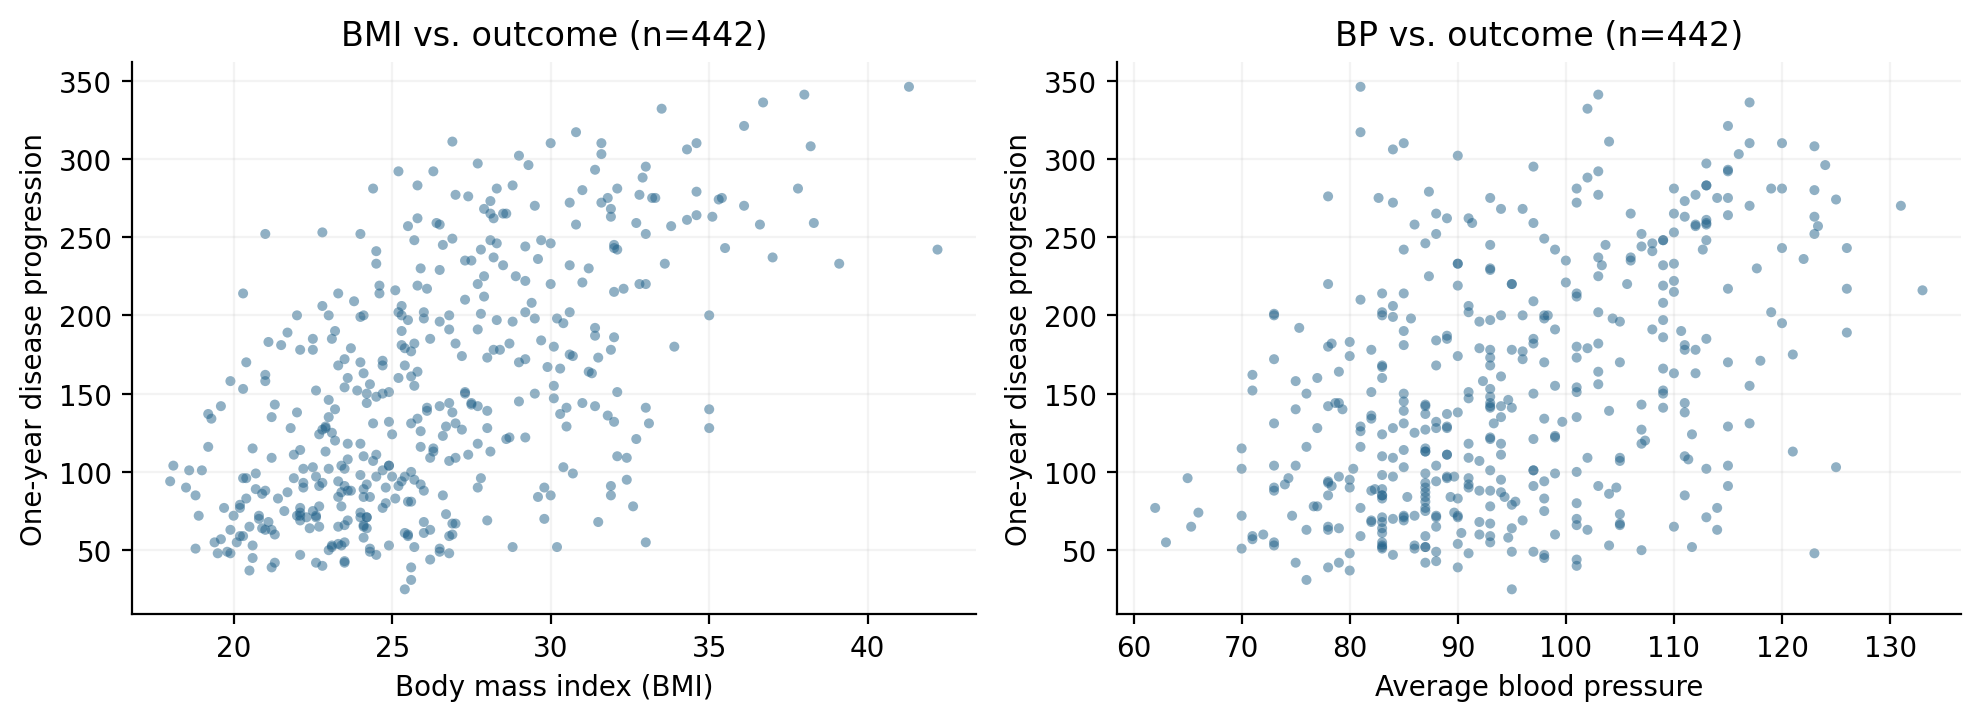
\includegraphics[width=0.94\textwidth,height=\textheight]{figures/fig01_diabetes_exploration.png}
\caption{Exploratory relationships of BMI and average blood
pressure with the continuous disease-progression target. Wide scatter
indicates that two predictors cannot explain all variation.}
\end{figure}

\textbf{Observation.} Higher BMI and higher blood pressure tend to
accompany higher progression scores, but both scatter plots show
substantial spread. This is an early indication that the two-feature
linear fit may have limited predictive accuracy.

\subsection{2.2 Dataset 2: Breast cancer diagnostic features (logistic
regression)}\label{dataset-2-breast-cancer-diagnostic-features-logistic-regression}

\textbf{Problem.} Classify pre-existing diagnostic feature records as
malignant or benign. The Wisconsin Diagnostic Breast Cancer dataset is
documented in the UCI Machine Learning Repository, in Street et
al.~(1993), and in the scikit-learn dataset guide {[}3--5{]}. It
contains 569 observations, including 212 malignant and 357 benign
samples. It contains 30 candidate features; this lab selects just two:
worst radius and worst concave points. These describe properties derived
from cell-nucleus images rather than clinical symptoms.

\textbf{Dataset provenance and interpretation.} The UCI repository
identifies these as measurements derived from digitized fine-needle
aspirate images of breast masses {[}3, 4{]}. Records in this experiment
are pre-extracted feature measurements, not raw images.

\textbf{Inputs and preprocessing.} The binary outcome is encoded
\textbf{1 = malignant}, \textbf{0 = benign}. This reverses the dataset's
original numeric label mapping to make sensitivity to malignancy
explicit. The split is stratified to preserve relative class
proportions. StandardScaler means and standard deviations are estimated
on training samples only. This dataset is suitable for logistic
regression because the outcome is binary and both selected predictors
are numerical.

\begin{figure}
\centering
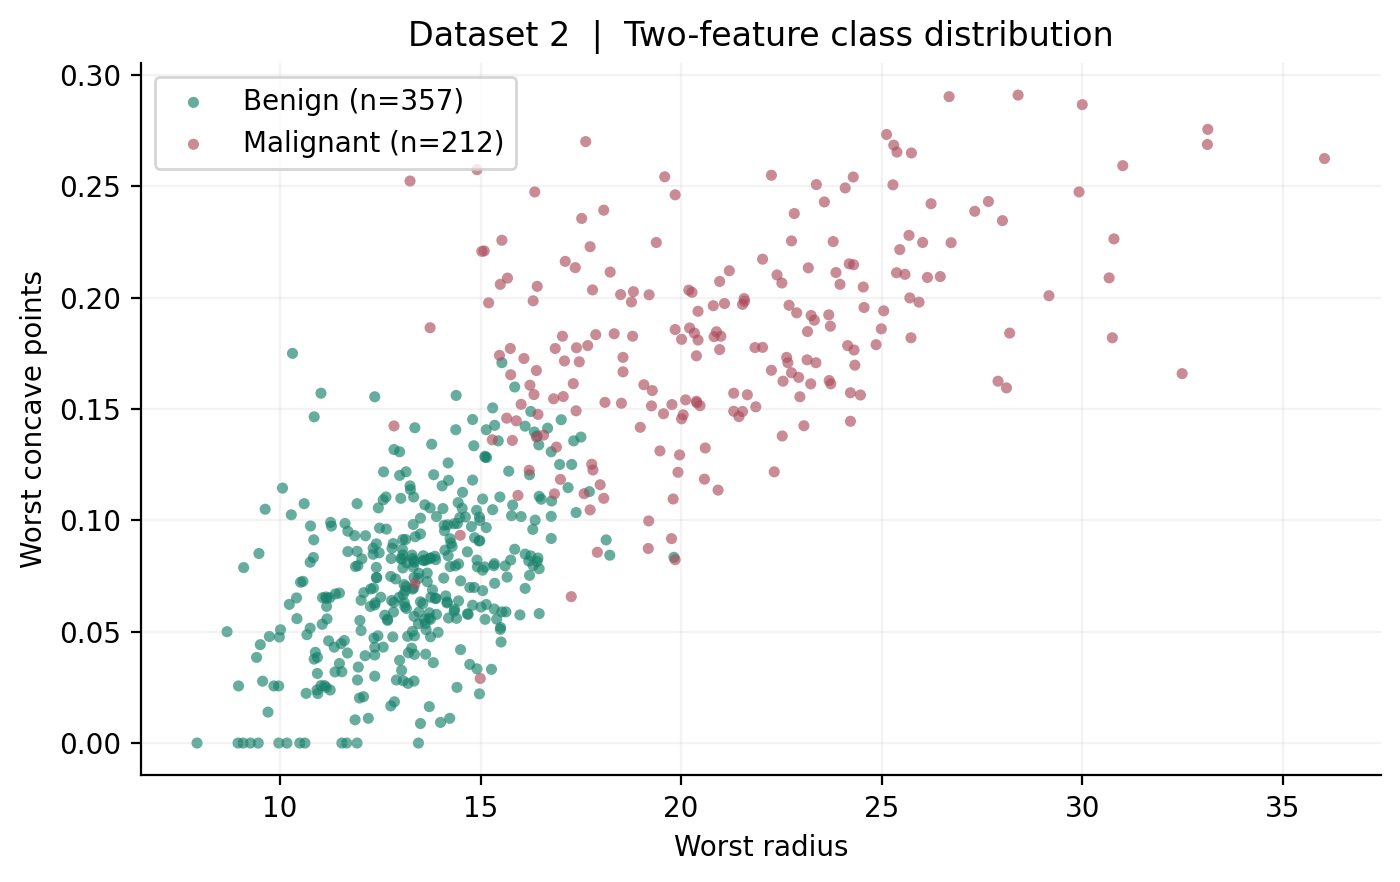
\includegraphics[width=0.86\textwidth,height=\textheight]{figures/fig05_breast_cancer_exploration.png}
\caption{Distribution of the 569 diagnostic records across the
two input features. The partially overlapping regions motivate
probabilistic classification.}
\end{figure}

\textbf{Observation.} Malignant observations tend to have larger values
of both features. The classes overlap, implying that no simple boundary
can eliminate every mistake without changing the balance between false
positives and false negatives.

\section{3. Part B --- Linear Regression
Experiments}\label{part-b-linear-regression-experiments}

\subsection{B1. Model parameters and
predictions}\label{b1.-model-parameters-and-predictions}

Ordinary least squares was fitted on the raw BMI and blood-pressure
values. The resulting linear model is an intercept plus one coefficient
for each input.

\begin{longtable}[]{@{}
  >{\raggedright\arraybackslash}p{(\columnwidth - 4\tabcolsep) * \real{0.3333}}
  >{\raggedleft\arraybackslash}p{(\columnwidth - 4\tabcolsep) * \real{0.3333}}
  >{\raggedright\arraybackslash}p{(\columnwidth - 4\tabcolsep) * \real{0.3333}}@{}}
\toprule\noalign{}
\begin{minipage}[b]{\linewidth}\raggedright
Fitted parameter
\end{minipage} & \begin{minipage}[b]{\linewidth}\raggedleft
Estimate
\end{minipage} & \begin{minipage}[b]{\linewidth}\raggedright
Meaning with other feature fixed
\end{minipage} \\
\midrule\noalign{}
\endhead
\bottomrule\noalign{}
\endlastfoot
Intercept & -215.053 & Prediction when BMI and BP are both zero (outside
the observed population) \\
BMI coefficient & +9.048 & +9.05 progression points per BMI unit \\
Blood pressure coefficient & +1.355 & +1.35 points per BP unit \\
\end{longtable}

\begin{longtable}[]{@{}lr@{}}
\toprule\noalign{}
Held-out test metric & Result \\
\midrule\noalign{}
\endhead
\bottomrule\noalign{}
\endlastfoot
Mean absolute error (MAE) & 50.044 \\
Mean squared error (MSE) & 3740.507 \\
Root mean squared error (RMSE; additional context) & 61.160 \\
Coefficient of determination (R\textsuperscript{2}) & 0.294 \\
\end{longtable}

\begin{figure}
\centering
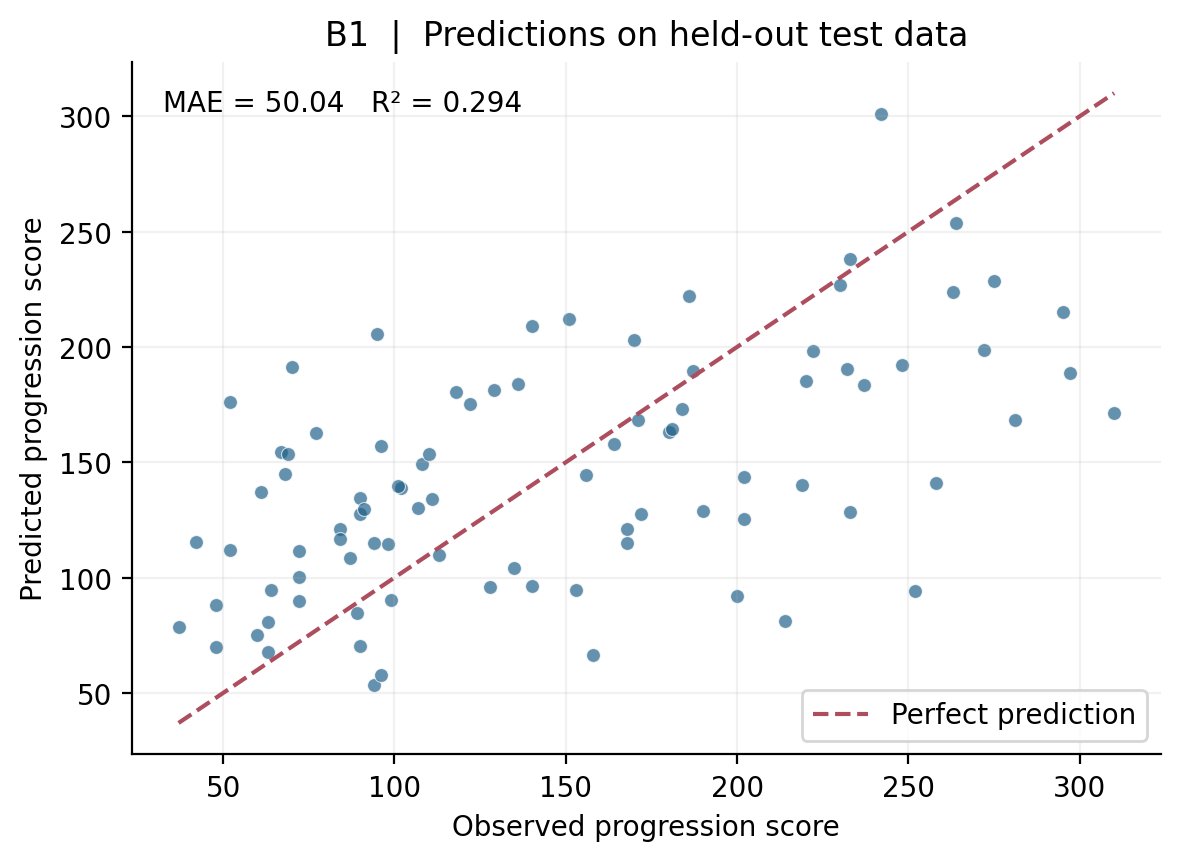
\includegraphics[width=0.77\textwidth,height=\textheight]{figures/fig02_regression_actual_predicted.png}
\caption{Actual versus predicted progression scores on the 89
held-out diabetes observations. The dashed diagonal denotes perfect
predictions.}
\end{figure}

\textbf{Interpretation.} Holding blood pressure constant, one higher BMI
unit is associated with about 9.05 higher predicted progression points,
whereas one higher BP unit is associated with about 1.35 higher points,
all else equal in this simple model. Because the feature units differ,
coefficient magnitudes should not be interpreted as direct rankings of
importance. The negative intercept is an extrapolation, not a physically
meaningful patient's score. Test MAE approximately 50.0 progression
points and R\textsuperscript{2} approximately 0.294 show moderate-to-weak explanatory
ability; predictions cluster toward the mean and miss extreme cases.
Association does not establish causation.

\subsection{B2. Feature scaling}\label{b2.-feature-scaling}

A second OLS model was trained after fitting StandardScaler \textbf{only
to the training set}. It subtracts training means and divides by
training standard deviations. For unregularized OLS with an intercept,
this affine transformation changes the numerical coefficients, but not
the set of fitted predictions.

\begin{longtable}[]{@{}lrr@{}}
\toprule\noalign{}
Comparison & Raw features & Standardized features \\
\midrule\noalign{}
\endhead
\bottomrule\noalign{}
\endlastfoot
BMI coefficient & 9.048 & 39.632 \\
Blood pressure coefficient & 1.355 & 19.043 \\
Intercept & -215.053 & 153.737 \\
Test MAE & 50.044 & 50.044 \\
Test R\textsuperscript{2} & 0.294 & 0.294 \\
\end{longtable}

\begin{figure}
\centering
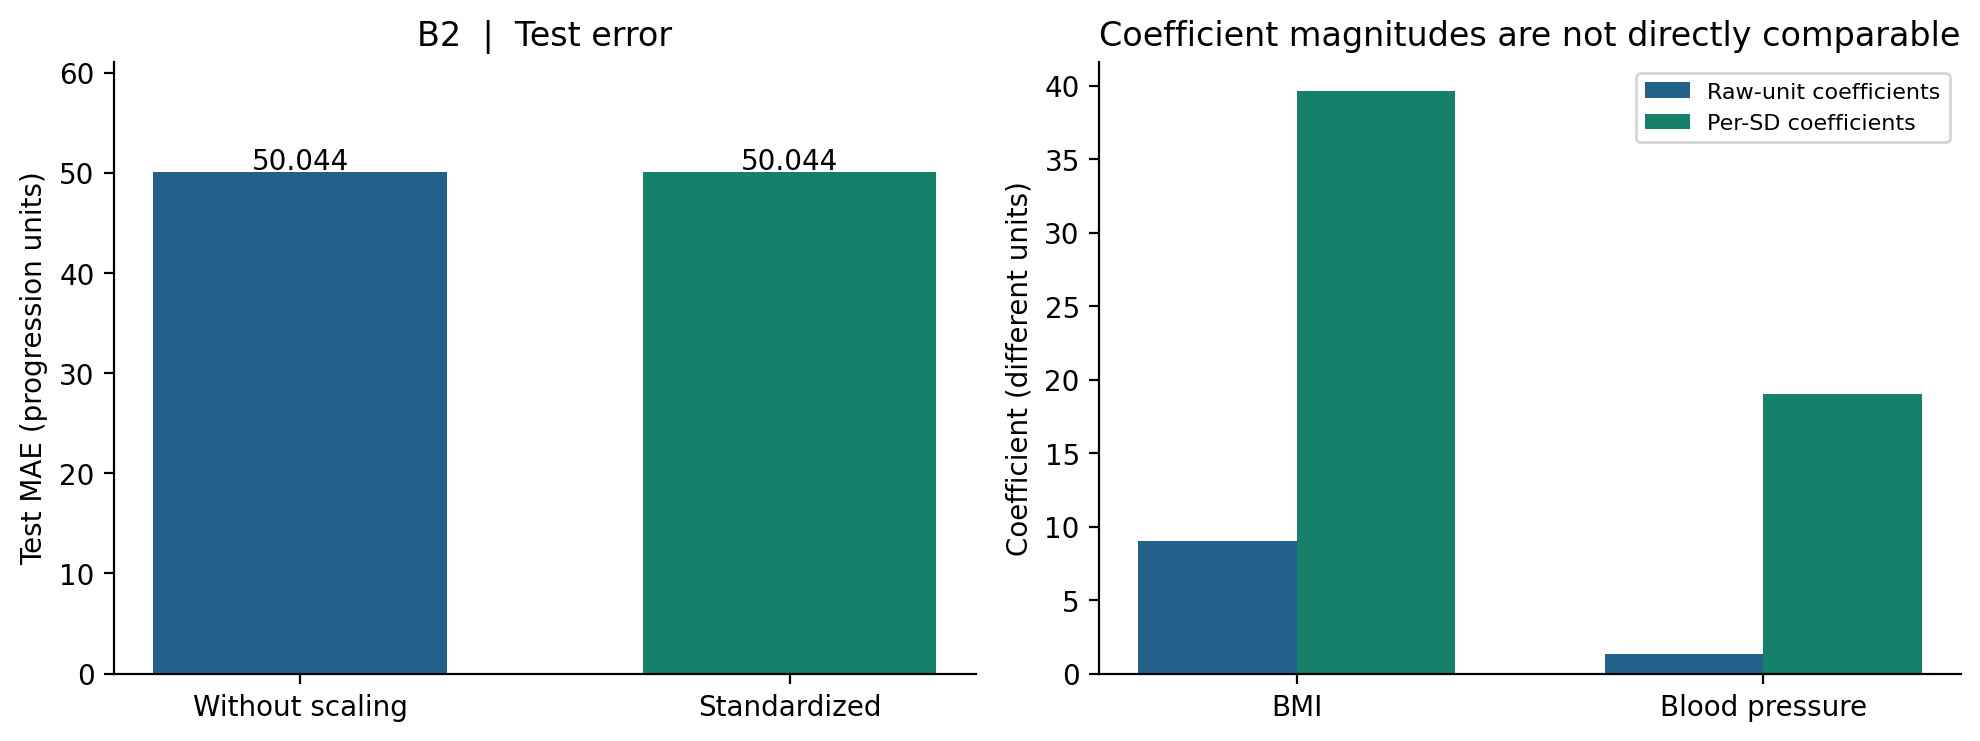
\includegraphics[width=0.94\textwidth,height=\textheight]{figures/fig03_scaling_comparison.png}
\caption{Baseline versus standardized OLS: identical test MAE,
despite changed coefficient scales. Coefficient groups use different
units and must not be compared directly.}
\end{figure}

\textbf{Interpretation.} The largest absolute difference between the two
models' test predictions was only 5.68e-14, attributable to
floating-point precision. After standardization, the BMI coefficient
represents one \textbf{training-set standard deviation} of BMI rather
than one BMI unit; the intercept becomes the predicted score at the
training feature means. Standardization matters especially to
gradient-based optimization, distance-based methods, and regularized
models, even though it leaves this OLS model's predictive accuracy
unchanged.

\subsection{B3. Learning rate and
convergence}\label{b3.-learning-rate-and-convergence}

To make learning behavior observable, batch gradient descent minimized
half the \textbf{training} mean squared error using the same
standardized diabetes features and centered training target. All runs
started with zero coefficients, used 150 iterations, and differed
\textbf{only} in learning rate ($\eta$). The exact OLS minimum of this same
objective was 1773.929 training-loss units. ``Within 1\%'' means the
first iteration at which the loss is no greater than 1.01 times that
minimum.

\begin{longtable}[]{@{}
  >{\raggedleft\arraybackslash}p{(\columnwidth - 6\tabcolsep) * \real{0.2500}}
  >{\raggedleft\arraybackslash}p{(\columnwidth - 6\tabcolsep) * \real{0.2500}}
  >{\raggedleft\arraybackslash}p{(\columnwidth - 6\tabcolsep) * \real{0.2500}}
  >{\raggedright\arraybackslash}p{(\columnwidth - 6\tabcolsep) * \real{0.2500}}@{}}
\toprule\noalign{}
\begin{minipage}[b]{\linewidth}\raggedleft
Learning rate ($\eta$)
\end{minipage} & \begin{minipage}[b]{\linewidth}\raggedleft
Loss at iteration 10
\end{minipage} & \begin{minipage}[b]{\linewidth}\raggedleft
Loss at iteration 150
\end{minipage} & \begin{minipage}[b]{\linewidth}\raggedright
First within 1\% of optimum
\end{minipage} \\
\midrule\noalign{}
\endhead
\bottomrule\noalign{}
\endlastfoot
0.01 & 2737.0 & 1802.1 & Not reached \\
0.10 & 1851.9 & 1773.9 & 17 \\
0.80 & 1773.9 & 1773.9 & 2 \\
1.50 & 8682.6 & 3.03e+14 & Diverges \\
\end{longtable}

\begin{figure}
\centering
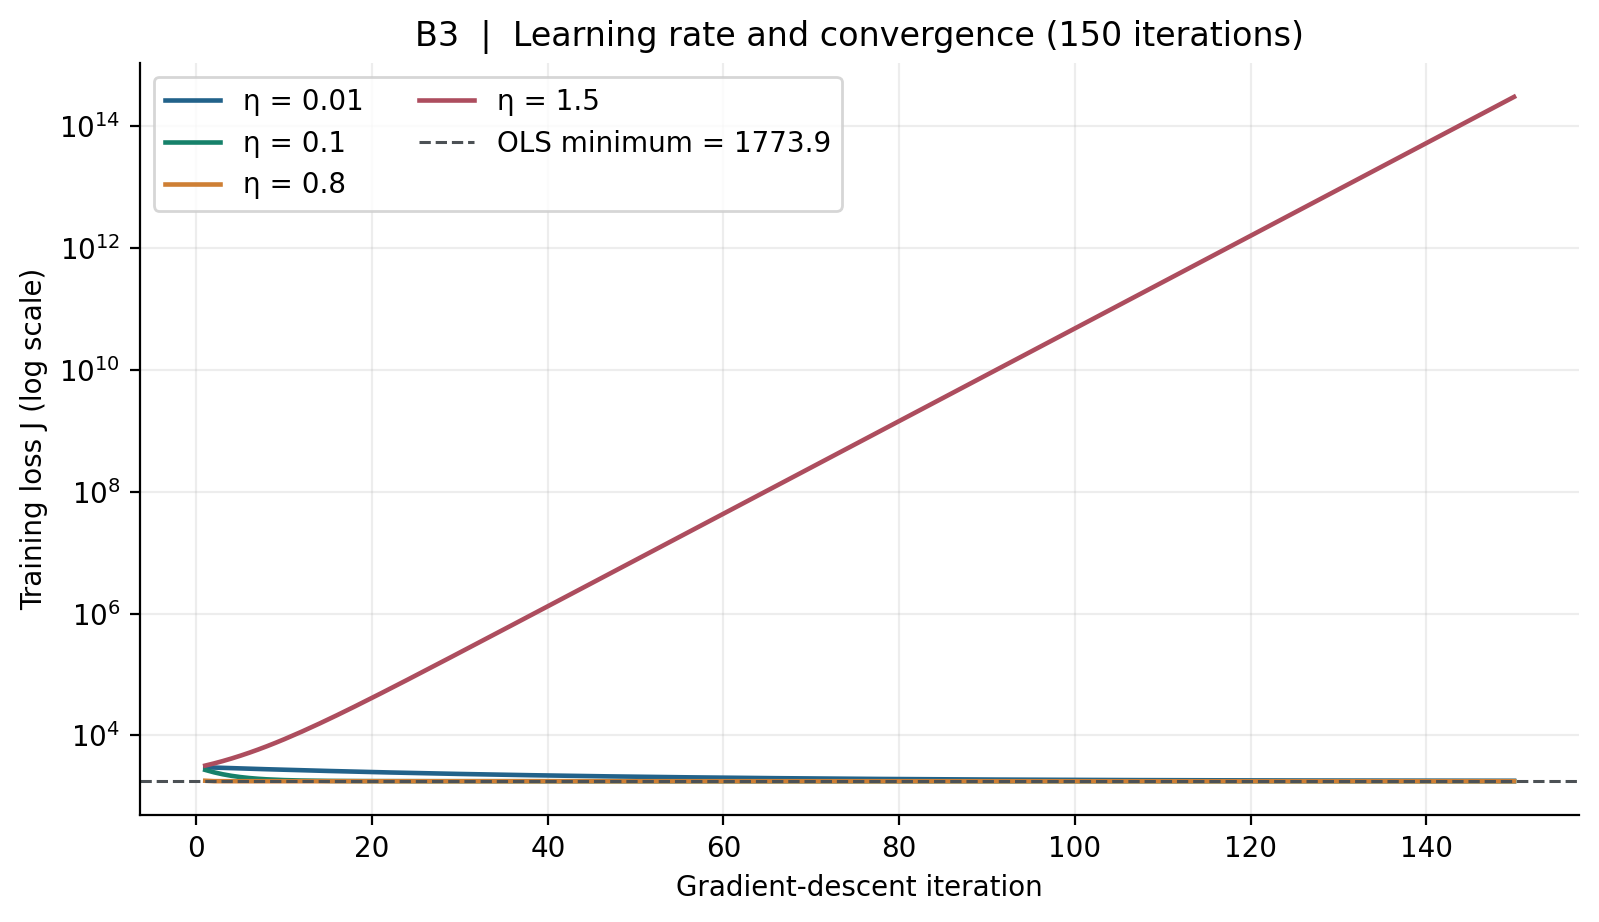
\includegraphics[width=0.91\textwidth,height=\textheight]{figures/fig04_learning_rate_convergence.png}
\caption{Training loss versus iteration for four learning
rates, shown on a log scale. $\eta$ = 0.80 converges rapidly; $\eta$ = 1.50
diverges.}
\end{figure}

\textbf{Interpretation.} Among tested values, $\eta$ = 0.80 was the fastest
stable choice, reaching the 1\% band after \textbf{2 iterations}. $\eta$ =
0.10 needed \textbf{17 iterations}, whereas $\eta$ = 0.01 remained outside
the band after 150 iterations. At $\eta$ = 1.50, the step size overshot
repeatedly and training loss grew to about 3.03e+14. More iterations can
help a stable small step, but cannot fix a divergent step. These
findings apply to this standardized two-feature quadratic objective, not
to every dataset.

\section{4. Part C --- Logistic Regression
Experiments}\label{part-c-logistic-regression-experiments}

\subsection{C1. Model parameters and binary
classification}\label{c1.-model-parameters-and-binary-classification}

The classifier uses a linear function of the two \textbf{standardized}
inputs, transformed by a sigmoid function into a probability of
malignancy. At threshold 0.5, probabilities at least 0.5 are labeled
malignant. An L2 penalty is applied by scikit-learn with C = 1.

\begin{longtable}[]{@{}
  >{\raggedright\arraybackslash}p{(\columnwidth - 4\tabcolsep) * \real{0.3333}}
  >{\raggedleft\arraybackslash}p{(\columnwidth - 4\tabcolsep) * \real{0.3333}}
  >{\raggedright\arraybackslash}p{(\columnwidth - 4\tabcolsep) * \real{0.3333}}@{}}
\toprule\noalign{}
\begin{minipage}[b]{\linewidth}\raggedright
Parameter (standardized model)
\end{minipage} & \begin{minipage}[b]{\linewidth}\raggedleft
Coefficient
\end{minipage} & \begin{minipage}[b]{\linewidth}\raggedright
Interpretation
\end{minipage} \\
\midrule\noalign{}
\endhead
\bottomrule\noalign{}
\endlastfoot
Worst radius & +3.269 & Higher standardized radius increases predicted
malignant log-odds \\
Worst concave points & +2.311 & Higher standardized concavity increases
predicted malignant log-odds \\
Intercept & -0.835 & Baseline log-odds at training mean feature
values \\
\end{longtable}

\begin{longtable}[]{@{}lr@{}}
\toprule\noalign{}
Test metric at threshold 0.5 & Result \\
\midrule\noalign{}
\endhead
\bottomrule\noalign{}
\endlastfoot
Accuracy & 0.956 (95.61\%) \\
Precision (malignant positive) & 0.974 \\
Recall / sensitivity & 0.905 \\
F1-score & 0.938 \\
True negative / false positive & 71 / 1 \\
False negative / true positive & 4 / 38 \\
\end{longtable}

\clearpage
\begin{figure}
\centering
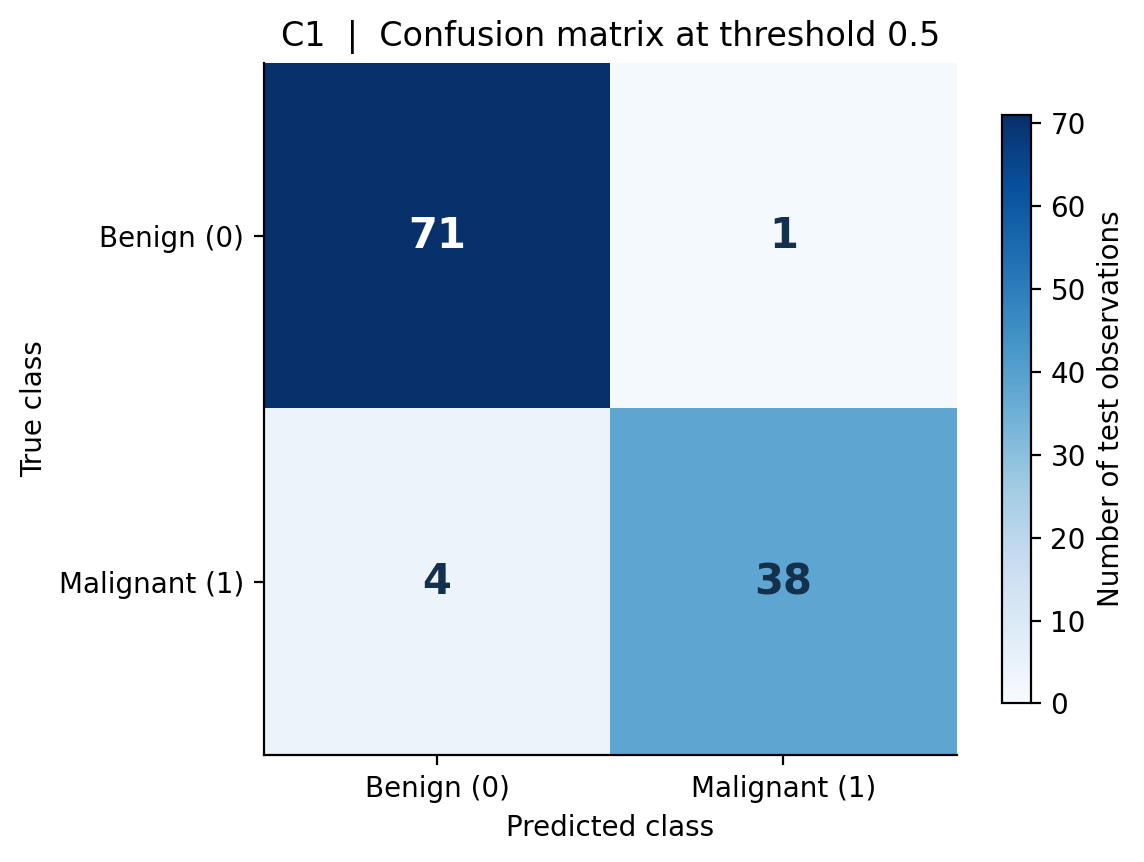
\includegraphics[width=0.75\textwidth,height=0.45\textheight,keepaspectratio]{figures/fig06_confusion_matrix.png}
\caption{Confusion matrix on the 114 held-out diagnostic
observations at threshold 0.5. Rows indicate actual diagnoses and
columns indicate predicted classes.}
\end{figure}

\textbf{Interpretation.} The raw linear score is a log-odds value; the
sigmoid produces a probability between 0 and 1 \textbf{before}
thresholding. A one-training-standard-deviation increase in worst
radius, with the other feature fixed, multiplies modeled odds by
approximately 26.27; the analogous factor for worst concave points is
10.09. These are model associations, not causal effects. The confusion
matrix shows \textbf{1 false positive} (benign labeled malignant) and
\textbf{4 false negatives} (malignant labeled benign). Missing malignant
cases is consequential in a hypothetical screening workflow, though this
dataset and model must \textbf{not} be interpreted as a validated
clinical tool.

\subsection{C2. Decision-threshold
experiment}\label{c2.-decision-threshold-experiment}

The logistic model was trained \textbf{once}. Exactly the same held-out
predicted probabilities were converted to labels using thresholds 0.3,
0.5, and 0.7; no refitting or new probability estimates were performed.

\begin{longtable}[]{@{}rrrrrrr@{}}
\toprule\noalign{}
Threshold & Accuracy & Precision & Recall & F1 & FP & FN \\
\midrule\noalign{}
\endhead
\bottomrule\noalign{}
\endlastfoot
0.3 & 0.974 & 0.933 & 1.000 & 0.966 & 3 & 0 \\
0.5 & 0.956 & 0.974 & 0.905 & 0.938 & 1 & 4 \\
0.7 & 0.930 & 1.000 & 0.810 & 0.895 & 0 & 8 \\
\end{longtable}

\begin{figure}
\centering
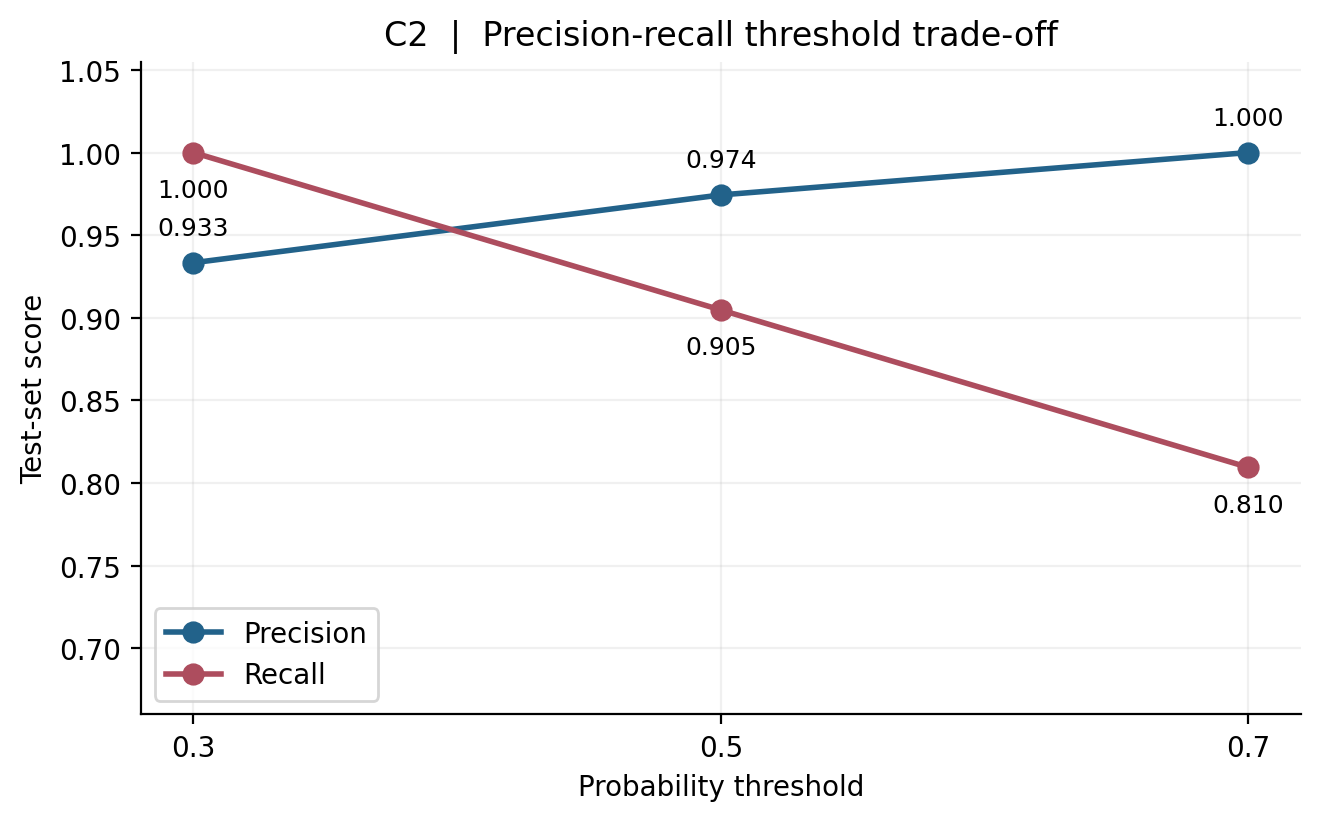
\includegraphics[width=0.81\textwidth,height=\textheight]{figures/fig07_thresholds.png}
\caption{Precision and recall evaluated on identical test
probabilities for three thresholds. A lower threshold emphasizes
sensitivity; a higher threshold emphasizes precision.}
\end{figure}

\textbf{Interpretation.} Lowering the threshold to 0.3 classified all 42
test malignant cases correctly (zero observed false negatives), at the
cost of 3 false positives. Raising it to 0.7 eliminated false positives
but increased false negatives to 8. For an illustrative high-sensitivity
triage setting, \textbf{0.3 is the preferred illustrative threshold}
among these options, because missing a positive is treated as more
costly than triggering follow-up review. This is \textbf{not a
clinically validated choice} and must not be selected for deployment
from test-set results: any genuine operating threshold should be fixed
on a separate validation set using explicit error costs, calibration,
and prospective evaluation.

\subsection{C3. One input feature versus two input
features}\label{c3.-one-input-feature-versus-two-input-features}

Two logistic models used the \textbf{same} training/test indices and
threshold 0.5: one used worst radius alone; the other included worst
radius and worst concave points. A fresh train-only scaler was fitted
within each model pipeline.

\begin{longtable}[]{@{}lrr@{}}
\toprule\noalign{}
Test metric & One feature & Two features \\
\midrule\noalign{}
\endhead
\bottomrule\noalign{}
\endlastfoot
Accuracy & 0.904 & 0.956 \\
Precision & 0.943 & 0.974 \\
Recall & 0.786 & 0.905 \\
F1-score & 0.857 & 0.938 \\
False negatives & 9 & 4 \\
\end{longtable}

\begin{figure}
\centering
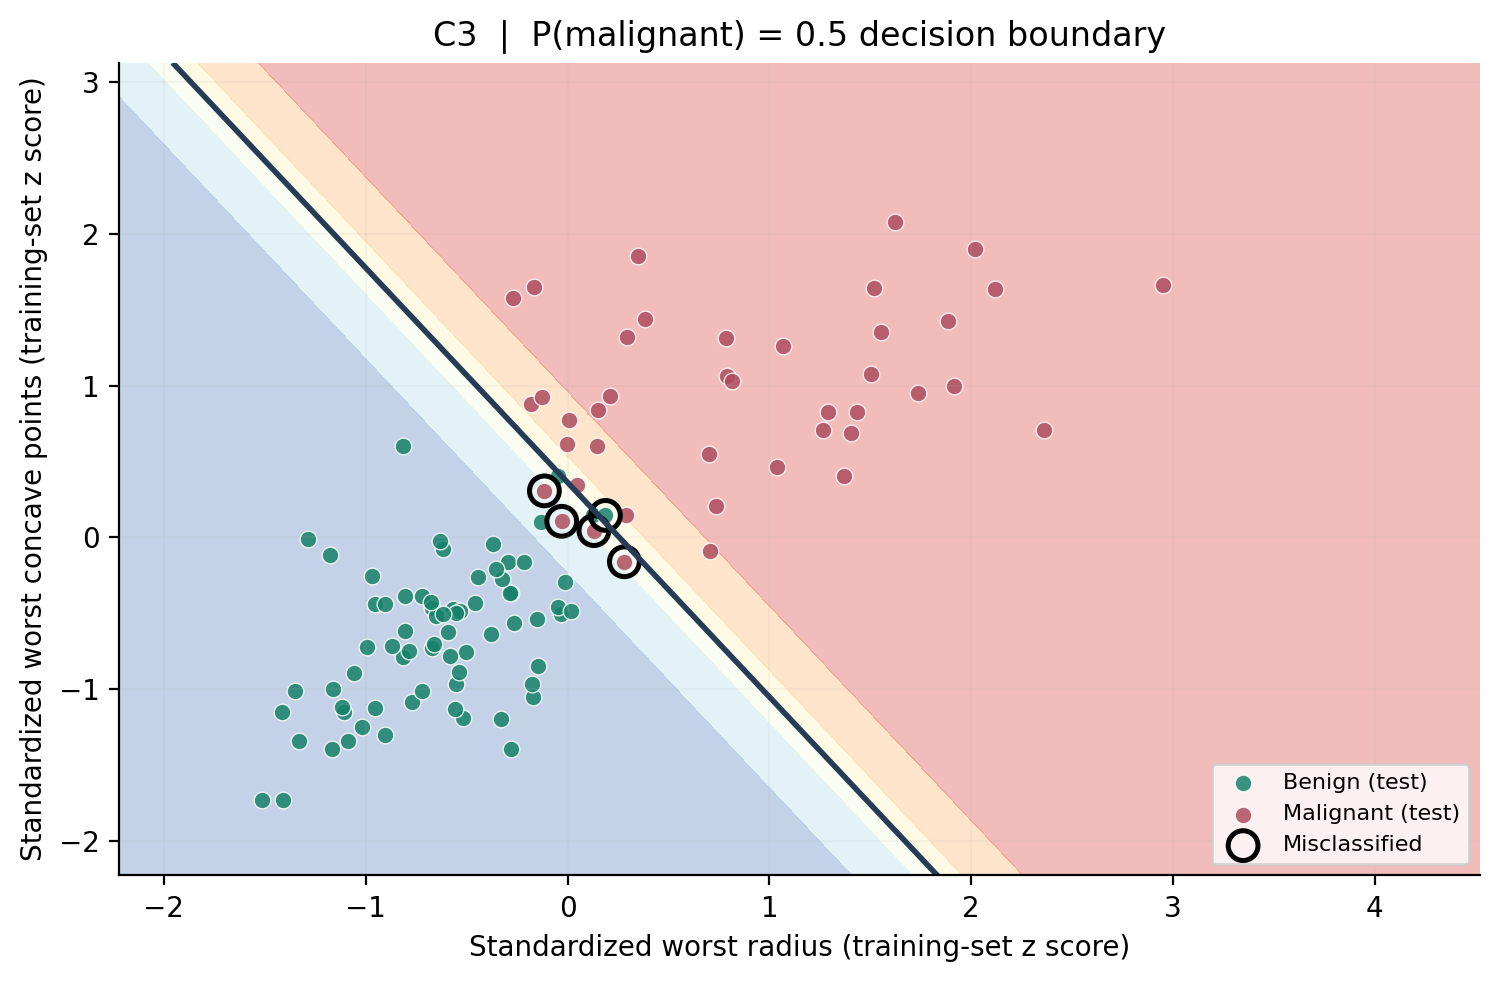
\includegraphics[width=0.91\textwidth,height=\textheight]{figures/fig08_decision_boundary.png}
\caption{Two-feature logistic decision boundary (dark line at
predicted probability 0.5) and held-out records in training-standardized
coordinates. Black rings mark test misclassifications.}
\end{figure}

\begin{figure}
\centering
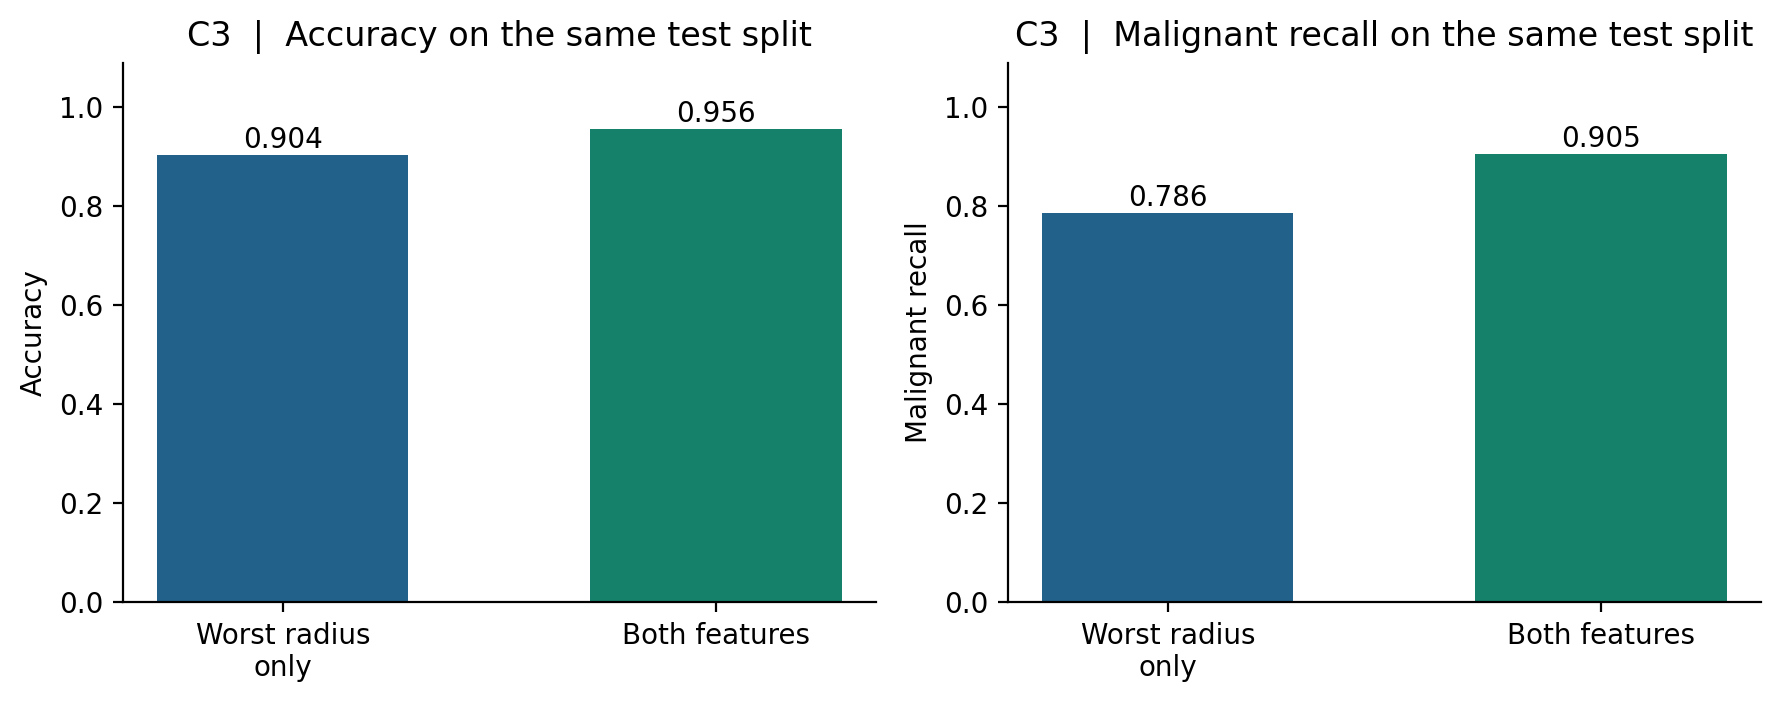
\includegraphics[width=0.91\textwidth,height=\textheight]{figures/fig09_one_vs_two_features.png}
\caption{Classification accuracy and malignant recall using
one feature versus both features on the identical held-out partition.}
\end{figure}

\textbf{Interpretation.} The second feature increased accuracy from
90.35\% to 95.61\%, while malignant recall increased from 0.786 to
0.905; false negatives decreased from 9 to 4. The decision boundary is
the set of feature combinations for which the model predicts 0.5
malignant probability. In these standardized two-dimensional coordinates
it is a straight line. Observations near the line and in overlapping
regions are difficult to classify because small changes in measured
features can flip the predicted label. Confident mistakes are also
possible when the two features omit useful information.

\section{5. Part D --- Reflection and
Comparison}\label{part-d-reflection-and-comparison}

\textbf{1. What differs between the two model outputs?} Linear
regression generates an unrestricted continuous prediction for a
numerical progression score. Logistic regression generates an estimated
\textbf{probability} of class 1 using a sigmoid; a chosen cutoff then
converts that probability to a benign/malignant decision. This
difference explains why B1 reports an MAE of 50.04 progression points
while C1 reports recall of 0.905 for malignant examples.

\textbf{2. What is a parameter versus a hyperparameter?} Parameters are
learned from training data: the BMI coefficient 9.048, the unscaled
regression intercept -215.053, and the standardized logistic coefficient
3.269 are examples. Hyperparameters are settings specified before
fitting, such as logistic C = 1, gradient-descent learning rate $\eta$, the
iteration count (150 in B3), and the classification cutoff. The cutoff
changes decisions, but not the fitted logistic coefficients.

\textbf{3. How does learning rate affect fitting?} A low rate moves
slowly ($\eta$ = 0.01 did not reach the 1\% training-loss band in 150
iterations), $\eta$ = 0.80 reached it in two, and $\eta$ = 1.50 diverged.
Iteration count and rate jointly control convergence; the largest step
is not always fastest in a stable sense.

\textbf{4. Why use different metrics?} Regression errors have a
magnitude in target units, so MAE, MSE, and R\textsuperscript{2} communicate numeric
performance. Classification errors are discrete and often have unequal
consequences. Accuracy alone hides the direction of errors; precision,
recall, F1, and the confusion matrix identify the trade-off. For
example, moving from threshold 0.5 to 0.7 raises malignant precision
from 0.974 to 1.000 but lowers recall from 0.905 to 0.810.

\textbf{5. What was unexpected?} Standardizing the OLS inputs
dramatically altered the numerical coefficients, while changing held-out
predictions by only 5.68e-14. This is explained by OLS being invariant
to invertible affine rescaling when an intercept is fitted. A second
informative result is that threshold 0.3 achieved zero false negatives
\textbf{on this particular test partition}; that result is not proof of
perfect sensitivity in unseen populations.

\section{6. Limitations and
Conclusion}\label{limitations-and-conclusion}

\textbf{Limitations.} The diabetes fit uses only two of ten available
predictors, yielding a modest R\textsuperscript{2}; omitted predictors, nonlinearity, and
measurement noise may account for residual errors. The cancer comparison
also uses just two of 30 features, evaluated on one stratified holdout
split (114 cases). A single split provides uncertain performance
estimates and the class frequencies may not reflect screening
populations. The threshold comparison is explanatory, not a valid
procedure for optimizing an operational cutoff on the test set. Neither
exercise performs patient-level external validation, fairness
assessment, probability calibration, or clinical risk analysis. No
medical decision should be based on these models.

\textbf{Conclusion.} The experiments demonstrate that model output
determines the appropriate learning objective and evaluation metrics.
OLS input standardization changes parameter units but not predictions,
whereas gradient descent shows strong sensitivity to step size. Logistic
classifications depend on both the learned probability surface and the
operating threshold. Adding a second diagnostic feature improved
held-out malignant recall in this study, yet careful validation is more
important than a single attractive test score.

\section{References}\label{references}

{[}1{]} Efron, B., Hastie, T., Johnstone, I., and Tibshirani, R. (2004).
``Least Angle Regression.'' \emph{The Annals of Statistics}, 32(2),
407--499. https://doi.org/10.1214/009053604000000067. (Original research
reference for the Diabetes data.)

{[}2{]} scikit-learn developers. (2026). ``Diabetes dataset ---
load\_diabetes.'' Official documentation.
https://scikit-learn.org/stable/modules/generated/sklearn.datasets.load\_diabetes.html
(accessed 21 October 2026). (Sample count, feature names, target
definition, and loader settings.)

{[}3{]} Wolberg, W., Mangasarian, O., Street, N., and Street, W. (1993).
\emph{Breast Cancer Wisconsin (Diagnostic)} {[}Data set{]}. UCI Machine
Learning Repository. https://doi.org/10.24432/C5DW2B. (Original dataset
citation, as provided by UCI.)

{[}4{]} Street, W. N., Wolberg, W. H., and Mangasarian, O. L. (1993).
``Nuclear feature extraction for breast tumor diagnosis.'' In
\emph{Biomedical Image Processing and Biomedical Visualization}, SPIE
Vol. 1905, 861--870. https://doi.org/10.1117/12.148698. (Study
describing source-image feature extraction.)

{[}5{]} scikit-learn developers. (2026). ``Breast cancer Wisconsin
dataset --- load\_breast\_cancer.'' Official documentation.
https://scikit-learn.org/stable/modules/generated/sklearn.datasets.load\_breast\_cancer.html
(accessed 21 October 2026). (Original class encoding, counts, and
input-feature dimensions.)

{[}6{]} Pedregosa, F., et al.~(2011). ``Scikit-learn: Machine Learning
in Python.'' \emph{Journal of Machine Learning Research}, 12,
2825--2830. https://jmlr.org/papers/v12/pedregosa11a.html. (Software
citation.)

\end{document}
